\renewcommand{\chaptername}{}

\setcounter{table}{0}
\renewcommand{\thetable}{B\arabic{table}}

\setcounter{figure}{0}
\renewcommand{\thefigure}{B\arabic{figure}}

\chapter{Appendix B: Additional literature review material} 
\label{sec:appendix2}

In their hybrid study of \textit{Dactylopius tomentosus} lineages, \citet{Mathenge2010} postulated that male and female crawlers might display differing host specifities due to the Comstockiella genetic system displayed in this insect family. In other words, males are haploid, containing only a maternal genome, while females are diploid with both a maternal and paternal genome. Taking such underlying genetic processes into account may be useful in explaining observed trends in inherited traits and the resulting host-specificity displayed by hybrid offspring. 

\section{The genetic system of the scale insects}
\label{appendix:geneticSystem}
The scale insects display one of the most diverse genetic and sex-determination systems of all the insects, including diploidy, parthenogenesis, hermaphroditism and haplodiploidy \citep{Burt2009,Ross2012}. The ancestral genetic system of scale insects is that of XX-XO (where 2n = 10), such that females are homogametic, and males are heterogametic with only one sex chromosome \citep{Hughes-Schrader1948, Nur}. 
Arrhenotoky and paternal genome elimination (PGE) (also termed ‘pseudoarrhenotoky’ or ‘parahaplodiploidy’) are variants of the haplodiploidy genetic system \citep{Haig1993,Gullan1997, Normark2004, Burt2009, Ross2010GenomicSystems}. To further complicate matters, the Hemiptera possess holocentric chromosomes, where spindle fibres attach along the length of the chromosome during cell division \citep{Hughes-Schrader1948}. This is in contrast to the typical monocentric chromosomes where spindle fibres attach to a single centromere \citep{Melters2012}. Holocentric chromosomes have allowed for a diverse range of karyotypes to form within the scale insects, such as species in the \textit{Apiomorpha} genus (Coccoidea: Eriococcidae) that display chromosome numbers from 2N = 4 to 2N = 92 \citep{Cook2000}. This is because if holocentric chromosomes become fragmented, all segments are pulled to opposite poles of the cell by spindle fibres during meiosis, as opposed to monocentric chromosomes that do not include fragmented sections and thereby maintain their original karyotype \citep{Melters2012}.  Additionally, scale insects display inverse meiosis \citep{Hughes-Schrader1948, Chandra1962, Bongiorni2004}. In this process, equational division occurs first followed by reduction division \citep{Wrensch1994, Bongiorni2004}. The difference between normal and inverse meiosis comes about due to the position of the paternal and maternal chromosomes relative to the orientation of the spindle fibres that form prior to metaphase I \citep{Wrensch1994} (Figure \ref{fig:meiosis}).

\vspace{1cm}

\begin{figure}[H]
	\centering
	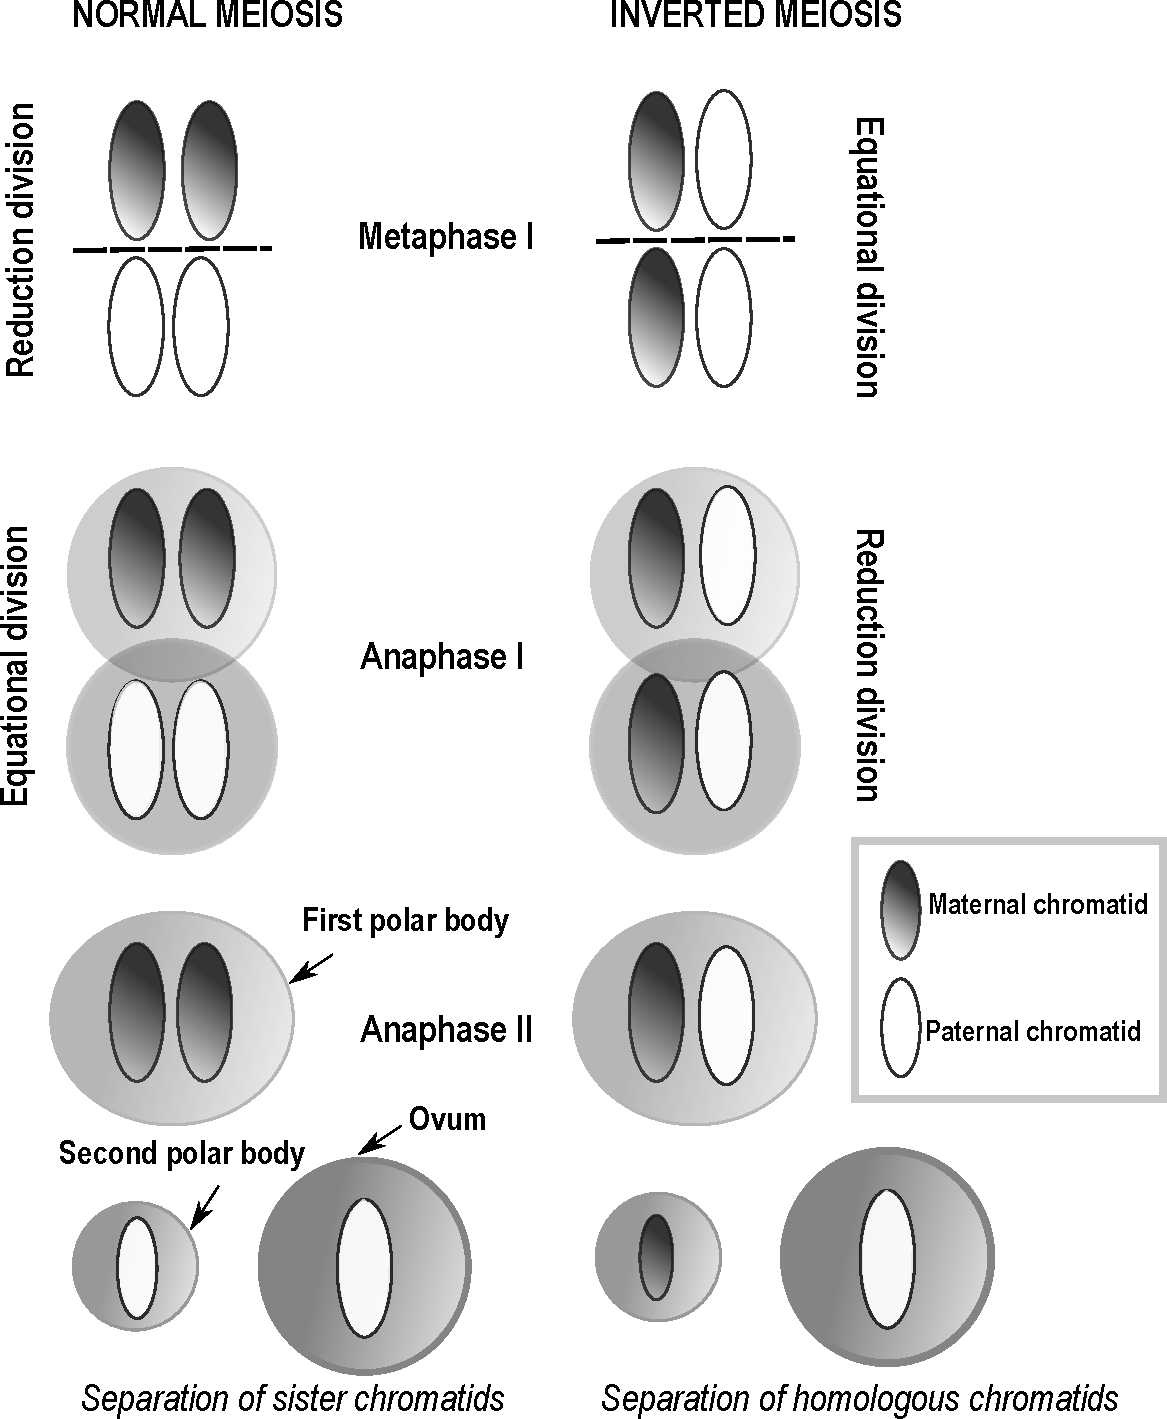
\includegraphics[scale = 0.6]{Images/meiosis.pdf}
	\caption{Difference between normal and inverted meiosis. Adapted from \citet{Brown1964, Wrensch1994, Bongiorni2004}}
	\label{fig:meiosis}
\end{figure} 

\subsection{The evolution of haplodiploidy}
Haplodiploidy refers to a genetic system where males are haploid and contain only a maternal genome, and females are diploid with both a maternal and paternal genome \citep{Normark2004, DelaFilia2015}. Haploidy in males occurs through either arrhenotoky (where females produce male offspring parthenogenetically) or PGE (where the paternal genome is eliminated at different developmental stages) \citep{Bull1979, Burt2009, Ross2010GenomicSystems}.
Haplodiploidy is present in as many as 15\% of arthropods \citep{DelaFilia2015}, and has evolved at least 10 times in insects \citep{Normark2004, Normark2006}. Why this system evolved is not well understood, but the leading hypotheses suggest the antagonistic co-evolution (intragenomic conflict) between the sexes, conflict over sex-determination, the clearance of deleterious mutations and rapid adaptation, and the role of endosymbionts (intergenomic conflict) in determining chromosome dynamics are possible drivers \citep{Normark2004, Burt2009, Ross2010GenomicSystems, DelaFilia2015}. 
\citet{Bull1979} and \citet{Herrick1999} suggested that maternal and paternal chromosomes engage in an arms race during spermatogenesis to transmit their genes to the next generation, and that this may explain the evolution of the different variations of PGE in scale insects. Females that produce haploid sons increase the transferal of their genes by two-fold in the gametes that their sons will produce \citep{Bull1979}. \citet{Normark2006} suggested that if an insect group displays gregariousness (as scale insects do), maternal care or other close kin associations, and relatedness asymmetry (i.e. offspring are linked more closely through their maternal line than through paternal genes), then offspring are more likely to display cooperative rather than competitive behaviour towards each other. In this case, some male genes may pose as selfish elements and can decrease overall fitness. \\
The sex determination system of scale insects that display PGE is poorly understood, with no record of the observation of sex chromosomes in species with this genetic system \citep{Brown1964, Ross2010GenomicSystems}. It is hypothesised that sex is determined by mechanisms such as gamete imprinting, the addition of maternal proteins to eggs \citep{Ross2010GenomicSystems}, the activity of endosymbionts \citep{Buchner1965}, and factors such as temperature \citep{Nelson-Rees1962}, population density, and the age of females at mating and oviposition \citep{Ross2010b}. Studies by \citet{Sabour1972} and \citet{Bongiorni2007} suggest that PGE and sex determination are maternally controlled through the production of histone proteins such as HP1, while \citet{Buglia2004} propose that it is the sperm that are tagged with proteins that determine sex. As an extension of intragenomic conflict between the sexes, haplodiploid fathers may favour a female-biased sex ratio, as this will ensure the transmittance of their genes to offspring \citep{DelaFilia2015}. This may lead to male selection for the manipulation of PGE dynamics \citep{DelaFilia2015}. Contrastingly, females may favour a male-biased sex ratio due to resource competition between daughters \citep{Taylor1981}. Since female scale insects are sessile and longer-lived in contrast to short-lived mobile males, females require more resources for survival and reproduction \citep{Taylor1981, Ross2010b}. \citet{Ross2010GenomicSystems}, for example, showed that \textit{Planococcus citri} (Coccoidea: Pseudococcidae) facultatively adjusted the sex ratio of offspring to favour males in response to high population densities. \\
Mutation rates and the efficiency of selection differentially affects haploid and diploid organisms \citep{Otto2008}. Relatively more mutations occur in diploids than haploids due to there being twice the number of genes available \citep{Mable1998, Otto2008, DelaFilia2015}. However, because of the capacity of homologous chromosome pairs to display heterozygosity, beneficial recessive mutations are masked and may take longer to become expressed in diploids \citep{Mable1998}. Additionally, the elimination of deleterious mutations through selection may be delayed due to this property \citep{Otto2008}. Because haploids immediately express mutations, deleterious mutations may be eliminated more efficiently, and beneficial mutations can spread more quickly through a haploid population \citep{DelaFilia2015}. Since haploid cells are generally smaller than diploid cells \citep{Galitski1999}, haploids have a higher surface area to volume ratio. It has therefore been suggested that haploid organisms have the ability to take in more nutrients across their cell membranes and have a higher chance of survival under nutrient-limited conditions \citep{Lewis1985}. Additionally, a smaller genome size could be less metabolically demanding \citep{Lewis1985}. \citet{Cavalier-Smith1978} suggested that smaller-bodied organisms, such as many endoparasites, tend to display haplodiploidy while larger-bodied organisms tend to be diploid due to differences in cell volume. \\
Scale insects feed on the phloem of their host plants, which is typically sugar-rich but nitrogen-poor \citep{Buchner1965, Douglas2006}. This has led to the evolution of obligate symbiotic relationships with microorganisms such as bacteria and unicellular fungi that synthesise amino acids and vitamins that their hosts can utilise \citep{Buchner1965,Douglas1998, Douglas2006, Douglas2015}. Endosymbiotic bacteria are usually housed in specialized organs called ‘bacteriomes’, in haemolymph, or inside modified fat cells within the insect host’s body \citep{Buchner1965, Normark2004b, Rosenblueth2018}. Bacteria are vertically transmitted to offspring via the maternal line in the cytoplasm of eggs \citep{Buchner1965, Rosenblueth2018}. Since males play no role in the transferal of bacteriomes, it is theorized that a potential intergenomic conflict exists between male hosts and endosymbionts regarding sex allocation \citep{Ross2010GenomicSystems}. Bacteria would favour a female-biased ratio to ensure their survival, while male insects would resist this pressure to prevent a reduction in paternal gene transfer to offspring \citep{Ross2010GenomicSystems}. In PGE systems however, male hosts and endosymbionts may have a shared interest in a female-biased sex ratio as males can only transmit their genes to female offspring, as discussed above \citep{Ross2010GenomicSystems}. Some studies have shown that symbionts can feminise \citep{Rigaud1997} and even kill males \citep{Hurst1991}, or induce parthenogenesis in their host \citep{Stouthamer1990}. 

\subsection{Paternal genome elimination}
Paternal genome elimination involves the deactivation and elimination of the paternal half of the genome through the process of heterochromatisation in male offspring \citep{Nur, Ross2010GenomicSystems}. As such, male sons transmit only their mother's genome to the next generation, making their closest male relatives their maternal grandfathers \citep{DelaFilia2015}. In this way, selection on male genes skips a generation \citep{DelaFilia2015}. At least 20 000 recorded species display PGE \citep{DelaFilia2015}, including more than half of the approximately 6000 known species of scale insects \citep{Burt2009}. It has also been recorded in some fungus gnats (\textit{Sciara} spp.) \citep{Haig1993b}, gall midges (\textit{Mayetiola destructor}) \citep{Haig1993}, phytoseiid mites (\textit{Amblyseius} spp.) \citep{Nelson-Rees1980}, springtails (\textit{Sminthurus viridis} and \textit{Allacma fusca}) (Collembola: Sminthuridae) \citep{Dallai2000} and a species of coffee borer beetle (Coleoptera: Scolytidae) (\textit{Hypothenemus hampei}) \citep{Brun1995}.
There are three different categories of PGE, depending on the timing of the elimination of the paternal set of chromosomes in male offspring \citep{Ross2010GenomicSystems}. These are namely the lecanoid, Comstockiella and diaspidid systems, where the Dactylopiidae family displays the Comstockiella PGE system \citep{Nur} (Figure \ref{fig:pge}). The lecanoid and Comstockiella systems are very similar, the only difference is that the paternal half of the genome is eliminated during the process of spermatogenesis in the former, and before meiosis in the latter \citep{Ross2010GenomicSystems}. In the lecanoid system, both the euchromatic maternal and heterochromatic (i.e. deactivated) paternal genomes undergo meiosis, but no crossing over occurs \citep{Burt2009}. The resulting sperm cells that receive the paternal heterochromatic set are non-functional \citep{Burt2009}. The Comstockiella system results in the full or partial elimination of the heterochromatic paternal genome prior to meiosis, where the number of paternal chromosomes that are eliminated can vary between species, individuals of the same species and even between different regions of testicular cyst tissue within an individual \citep{Burt2009}.
The Diaspidid system has only been recorded in the Diaspididae family (the armored scale insects) \citep{Nur, Ross2010GenomicSystems, Burt2009}. In this system, instead of being deactivated, the paternal chromosomes are destroyed during embryogenesis, rendering males haploid throughout their lives \citep{Ross2010GenomicSystems}. 
This process could have been selected for as an energy-saving strategy to eliminate the need of replicating deactivated chromosomes, and as a means of preventing their potential reactivation \citep{Burt2009}. \citet{Nur1967}, for example, found that the male genome of the citrus mealybug \textit{Planococcus citri} (Hemiptera: Pseudococcidae) became reactivated in some tissues, including reproductive cyst tissue where spermatogenesis takes place.
\vspace{0.4cm}

\begin{figure}[H]
	\centering
	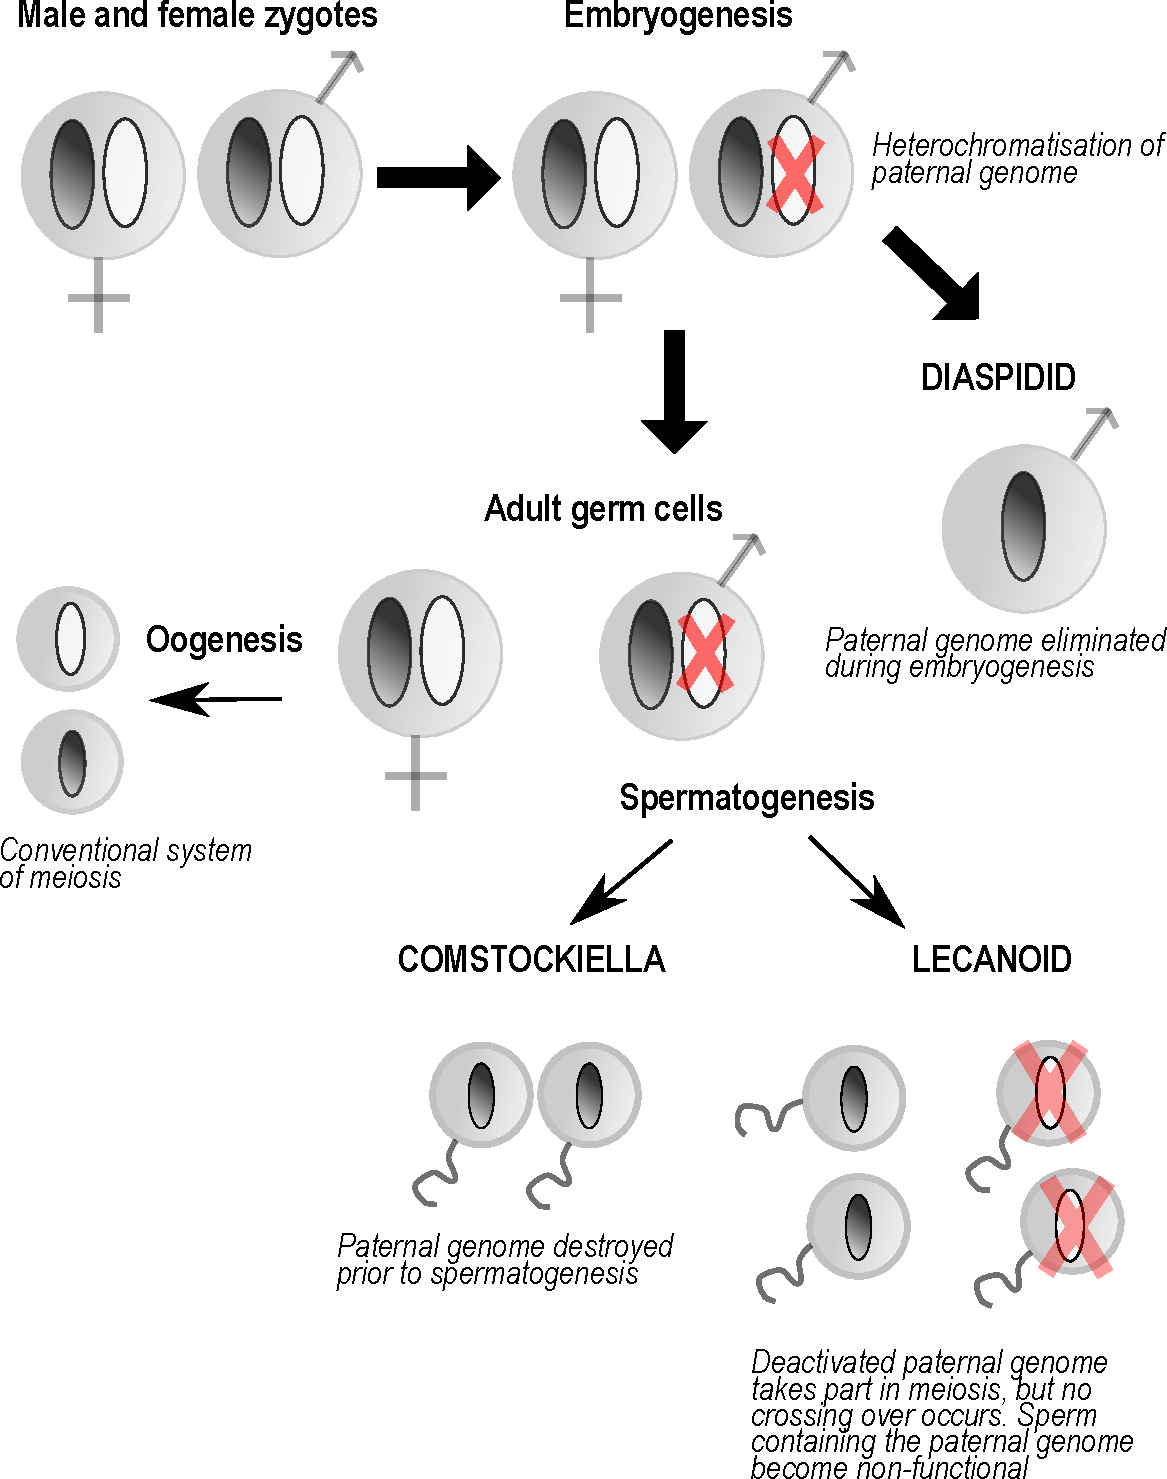
\includegraphics[scale = 0.6]{Images/PGE_system.pdf}
	\caption{Paternal genome elimination in scale insects, showing the lecanoid, diaspidid and Comstockiella  genetic systems. Adapted from \citet{Bull1979, Burt2009, Ross2010GenomicSystems}}
	\label{fig:pge}
\end{figure} 

\section{Life cycle of the Dactylopiidae}
\label{appendix:lifecycle}
\citet{Perez-Guerra1992} undertook a detailed study of the life history of \textit{D. coccus}, which is representative of the genus. Males undergo six life stages (egg $\rightarrow$ first instar $\rightarrow$ second instar $\rightarrow$ pre-pupa $\rightarrow$ pupa $\rightarrow$ winged adult), while females undergo four (egg $\rightarrow$ first instar $\rightarrow$ second instar $\rightarrow$ sessile adult female). Oviposition usually occurs at night. Eggs are a light red colour and either hatch within the female (ovoviviparity), or within ten to thirty minutes after oviposition, yielding red nymphs (referred to as `crawlers') approximately 1 mm in length \citep{Nobel2002CactiUses}. Both male and female crawlers begin producing waxy filaments within an hour of hatching to assist in wind dispersal. Following attachment to a host plant, female nymphs produce a dense protective waxy layer after the second moult. Adult females lay an average of approximately 430 eggs in their lifetime, that they oviposit in chain-like formations on the surface of the host plant. Males display a holometabolous-like life cycle, which incorporates a pre-pupal and pupal stage, giving rise to winged adults \citep{Nobel2002CactiUses}. Adult males do not feed, mate with multiple females, and live for approximately 50 to 80 days. Females are significantly longer-lived than males, living for up to five months \citep{Moran1979, Nobel2002CactiUses}.
\vspace{0.4cm}

\begin{figure}[H]
	\centering
	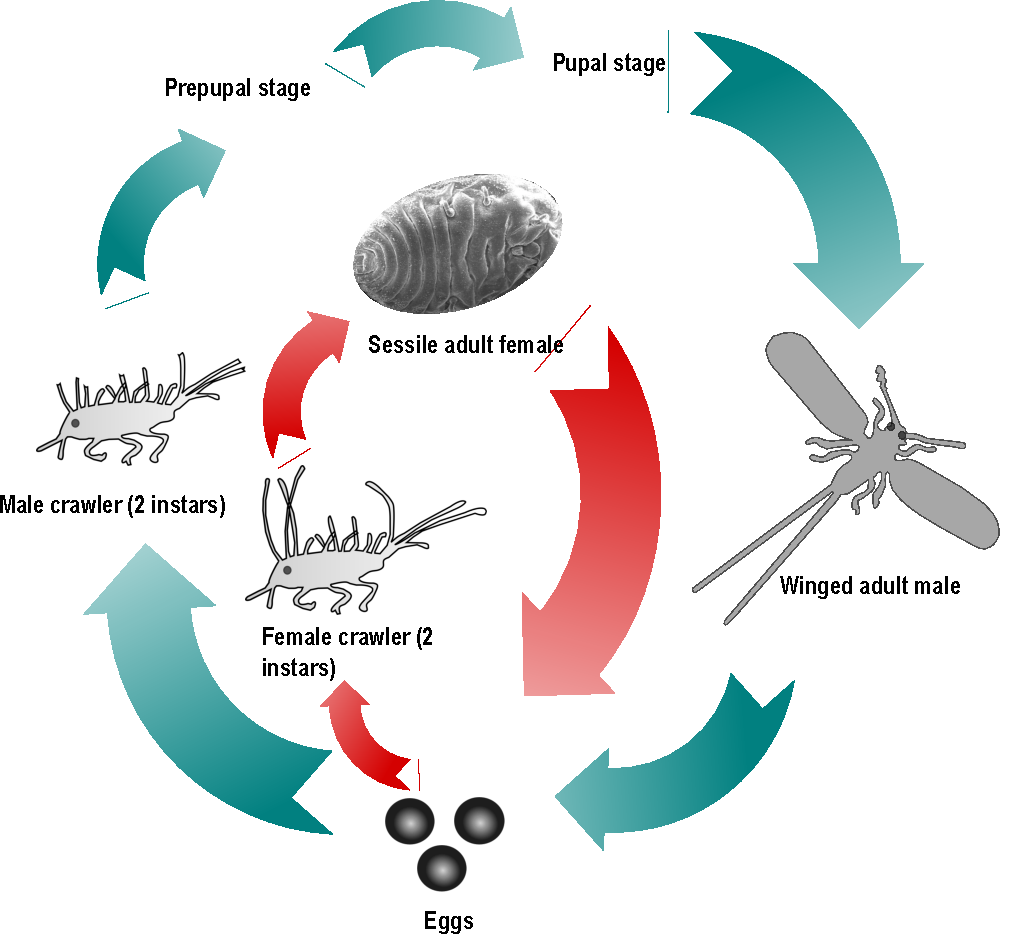
\includegraphics[scale = 0.65]{Images/lifecycle.pdf}
	\caption{Lifecycle of \textit{Dactylopius}. Adapted from \citet{Moran1979}}
	\label{fig:lifecycle}
\end{figure}

\begin{landscape}

\section{Genetic barcoding application examples}

	\renewcommand{\arraystretch}{0.5} % changes the linespacing
	\begin{longtable}{p{0.2\textwidth}p{1.2\textwidth}} 
		\caption{Cross-disciplinary examples of genetic barcoding} \label{tab:barcoding} \\	
		\toprule
		\multicolumn{1}{l}{\textbf{}} & \multicolumn{1}{c}{\textbf{Details}} \\ \midrule
		\multirow{2}{*}{Medicine} & Identification of the vertebrate hosts of haematophagous arthropods to better understand the ecology of host-parasite interactions and the implications for human and veterinary epidemiology \citep{Alcaide2009} \\ \cmidrule(l){2-2} 
		& Identification of sandfly (Diptera: Psychodidae) species in Columbia- vectors of Leishmania parasites \citep{Gutierrez2014} \\ \midrule
		\multirow{3}{*}{Agriculture} & Barcoding of the Heliothinae family to enable a method of rapid identification of potential crop pests entering Australia, particularly \textit{Helicoverpa} Hardwick spp. and \textit{Heliothis} Ochsenheimer spp \citep{Ball2006} \\ \cmidrule(l){2-2} 
		& Identification of two species of \textit{Busseola} (Lepidoptera: Noctuidae)- important pests of sugarcane in Ethiopia \citep{Assefa2007} \\ \cmidrule(l){2-2} 
		& Identification of invasive \textit{Spodoptera} (Lepidoptera: Noctuidae) in North America \citep{Nagoshi2011} \\ \midrule
		\multirow{4}{*}{Ecology} & Barcoding of scats, hair, blood, tissue and regurgitates to determine the presence and dispersal of wolves recolonizing the western Alps as well as assigning haplotypes to different source populations \citep{Valiere2003} \\ \cmidrule(l){2-2} 
		& Detecting the presence of a particular species of frog, \textit{Rana catesbeiana} Shaw, in water samples taken from freshwater environments \citep{Ficetola2008} \\ \cmidrule(l){2-2} 
		& Determination of the diet of \textit{Architeuthis} spp. The gut contents of a deep sea giant squid revealed the presence of \textit{Macruronus novaezelandiae} Hector, and also indicated that cannibalism occurs in this squid genus \citep{Deagle2005} \\ \cmidrule(l){2-2} 
		& Analysing ‘dirt DNA’ from soil samples as an indication of the vertebrate biodiversity in an area. The study concluded that the barcoding of eDNA can be an accurate measure of taxonomic richness and the relative biomass of species \citep{Andersen2012} \\ \midrule
		\multirow{4}{*}{Forensic science} & Detection of hairs from the protected Eurasian badger, \textit{Meles meles} L., in shaving brushes produced in the Netherlands, France, Italy, the UK and Spain \citep{Domingo-Roura2006} \\ \cmidrule(l){2-2} 
		& Uncovering the mislabeling of seafood in restaurant outlets. Sushi restaurants sampled in Los Angeles were shown to have a mislabeling percentage of 47\%, particularly regarding yellowfin tuna, yellowtail, Halibut and red snapper fish \citep{Willette2017} \\ \cmidrule(l){2-2} 
		& Uncovering of illegal trade (by means of sampling sushi) in protected fin, sei and Antarctic minke whales between Japan and the USA and South Korea \citep{Baker2010} \\ \cmidrule(l){2-2} 
		& Use of COI genetic barcoding to identify all the immature life stages of \textit{Sarcophaga impatiens} Walker (Diptera: Sarcophagidae); an important insect in forensic entomology \citep{Meiklejohn2013} \\ \midrule
		\multirow{2}{*}{Invasion biology} & Use of COI and 16S barcoding regions to identify diapausing eggs in ballast water. 64\% of the 96 samples were successfully identified to species level \citep{Briski2011} \\ \cmidrule(l){2-2} 
		& Test of different plant barcoding genes to determine the highest hit rate for the identification of invasive plants in China. It was found that ITS and matK markers were the most effective \citep{Xu2017} \\ \midrule
		\multirow{2}{0cm}{Paleontology and paleoecology} & Analysis of the diet  of \"{O}Ötzi-  the 5000 year old Neolithic mummy found in the Alps in 1991. The DNA barcoding results revealed that the man had eaten red deer (\textit{Cervus elaphus} L.), ibex (\textit{Capra ibex} L.) and cereals shortly before death. Pollen grains indicated that he must have passed through a subalpine forest during his journey \citep{Rollo2002} \\ \cmidrule(l){2-2} 
		& Analysis of permafrost sediment cores from Siberia (dating from the present to $\sim$1.5 to 2 million years ago), and cave and coastal sediments from New Zealand (dating back $\sim$600 to 3000 years). Results revealed large scale changes in plant and faunal diversity and composition over time, as well as the presence of extinct megafauna such as ratite moas in New Zealand, and mammoths, bison and horses in Siberia \citep{Willerslev2003} \\ \bottomrule
		
	\end{longtable}
\end{landscape}

\section{ISSR concept}
\begin{figure}[H]
	\centering
	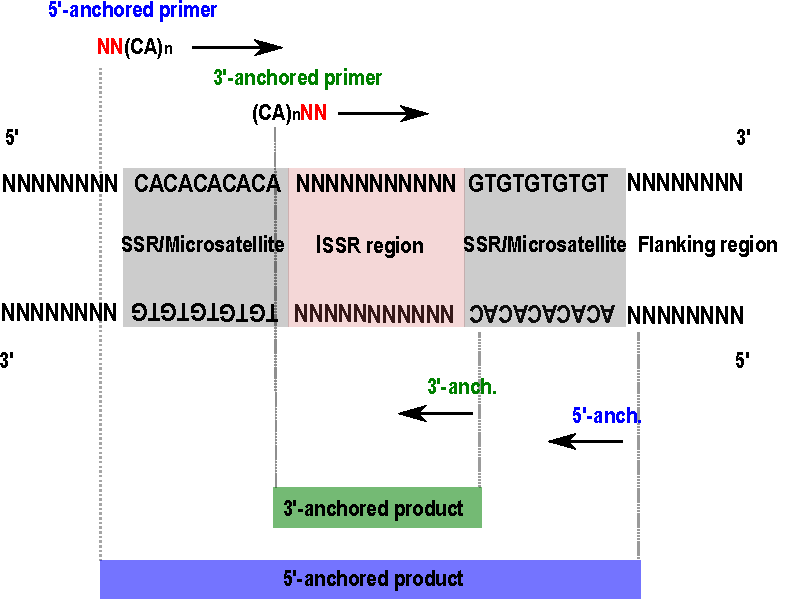
\includegraphics[scale = 1]{Images/issr.pdf}
    \newline
	\caption{An illustration of the concept of ISSR-PCR showing the use of 3' and 5'-anchored primers. A 5’-anchored primer attaches to the flanking region of a microsatellite, where a 3’-anchored primer attaches to the microsatellite region flanking the ISSR and forms a shorter PCR product. The ISSR region varies in size at different loci in the genome, producing unique banding patterns for each unique individual. Diagram adapted from \citet{Zietkiewicz1994,Reddy2002,Ng2015Inter-SimpleRight}.} 
	\label{fig:issr}
\end{figure}